\documentclass{article}

\usepackage{siunitx}
\usepackage{booktabs}
\usepackage{graphicx}
% \usepackage{minted}

\frenchspacing
\setlength{\parindent}{0ex}
\setlength{\parskip}{2 ex plus 2 ex minus 1 ex}

\title{Homework 2}
\author{Josh Bradt}
\date{February 1, 2016}

\begin{document}

\maketitle

\section{Array copy performance}

I ran this test on my Late-2012 Mac Mini with a quad-core, \SI{2.3}{GHz} Intel Core i7-3615QM processor. This processor has \SI{64}{kB} L1 cache per core, \SI{256}{kB} L2 cache per core, and \SI{6}{MB} L3 cache which is shared between the cores. The computer has \SI{16}{GB} of RAM installed. The operating system is Mac OS X El Capitan (10.11.2).

All codes were compiled using the default Apple-provided Clang version 7.0.2 with optimization level -O2.

The results for this section are shown in Table~\ref{tab:part1}. Note that I was unable to run the test for an array size of \num{5000000} since OS X sets a hard limit of \SI{65532}{kB} on the stack size which cannot be bypassed with \texttt{ulimit -s}.

\begin{table}[b]
\centering
\begin{tabular}{@{}rcc@{}}
\toprule
N         & Time for Loop (s) & Rate (MB/s) \\ \midrule
\num{250}       & \num{4.76E-08}          & \num{8.40E+04}    \\
\num{1000}     & \num{1.80E-07}          & \num{8.89E+04}    \\
\num{5000}     & \num{1.85E-06}          & \num{4.33E+04}    \\
\num{10000}    & \num{3.63E-06}          & \num{4.41E+04}    \\
\num{50000}    & \num{2.28E-05}          & \num{3.51E+04}    \\
\num{100000}   & \num{4.52E-05}          & \num{3.54E+04}    \\
\num{500000}   & \num{3.68E-04}          & \num{2.17E+04}    \\
\num{1000000} & \num{8.78E-04}          & \num{1.82E+04}    \\
\num{5000000} & (Failed)          & (Failed)    \\ \bottomrule
\end{tabular}
\caption{Results from Part 1}
\label{tab:part1}
\end{table}

The time results are plotted in Fig.~\ref{fig:p1time}, and the data rates are plotted in Fig.~\ref{fig:p1rate}.

\begin{figure}
    \centering
    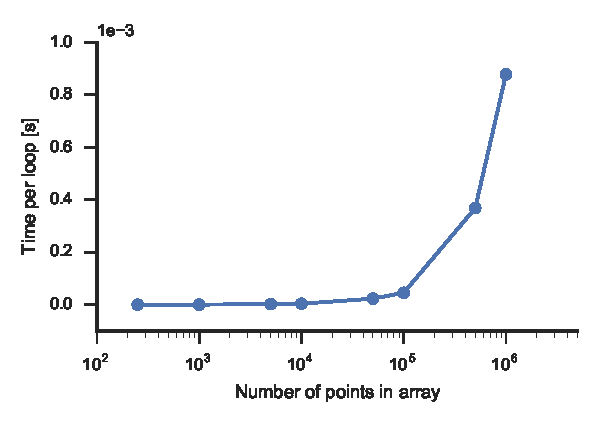
\includegraphics{p1time.pdf}
    \caption{Time per loop for Part 1.}
    \label{fig:p1time}
\end{figure}
\begin{figure}
    \centering
    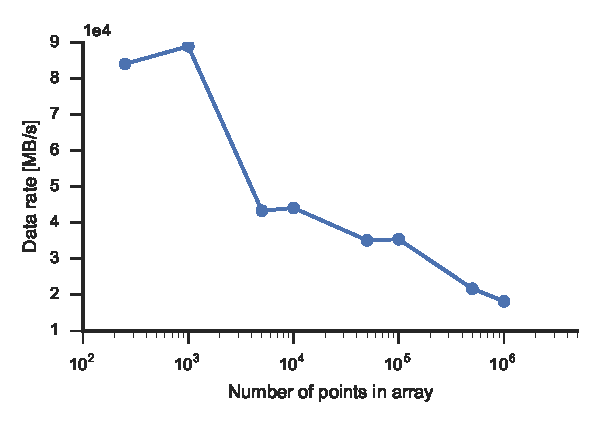
\includegraphics{p1rate.pdf}
    \caption{Data rate for Part 1.}
    \label{fig:p1rate}
\end{figure}

\section{STREAM benchmark}

I ran the C version of the STREAM benchmark on the same system as above, compiled as above with \texttt{clang -O2}. The array size was set to \num{3000000}, which produced an array size of \SI{22.9}{MiB}. This is more than 4 times the size of the \SI{6}{MB} L3 cache on this system.

The results of the benchmark are shown in Table~\ref{tab:stream}.

\begin{table}[]
\centering
\begin{tabular}{@{}rrrrr@{}}
\toprule
\textbf{Function} & Best rate {[}GB/s{]} & Avg time {[}ms{]} & Min time {[}ms{]} & Max time {[}ms{]} \\ \midrule
\textbf{Copy}     & 16.5                 & 3.14              & 2.89              & 4.12              \\
\textbf{Scale}    & 12.3                 & 4.25              & 3.92              & 5.28              \\
\textbf{Add}      & 12.7                 & 5.99              & 5.67              & 6.41              \\
\textbf{Triad}    & 12.7                 & 6.09              & 5.66              & 6.62              \\ \bottomrule
\end{tabular}
\caption{STREAM results}
\label{tab:stream}
\end{table}

\section{Sparse matrix-vector multiply performance estimate}

Based on the analysis in Lecture 4, the processor needs to load approximately 1 double and 1 integer for each floating point operation (assuming a single operation for multiply-add). This amounts to \SI{12}{B/FLOP}.

The STREAM results show that the processor can move about \SI{16.5}{GB/s} to or from memory. If the clock frequency is \SI{2.3}{GHz}, then this is \SI{7.2}{B/cycle}. Assuming the processor can perform \SI{1}{FLOP/cycle}, this means that it can move \SI{7.2}{B/FLOP}.

Thus, the expected performance is $(\SI{7.2}{B/FLOP}) / (\SI{12}{B/FLOP}) = \SI{60}{\percent}$ of the peak performance. This equals $0.6 \times \SI{2.3}{GFLOPS} = \SI{1.38}{GFLOPS}$.


\end{document}
